% Options for packages loaded elsewhere
\PassOptionsToPackage{unicode}{hyperref}
\PassOptionsToPackage{hyphens}{url}
%
\documentclass[
]{article}
\title{clusterGeneration Notes}
\author{Emily Raney}
\date{11/9/2022}

\usepackage{amsmath,amssymb}
\usepackage{lmodern}
\usepackage{iftex}
\ifPDFTeX
  \usepackage[T1]{fontenc}
  \usepackage[utf8]{inputenc}
  \usepackage{textcomp} % provide euro and other symbols
\else % if luatex or xetex
  \usepackage{unicode-math}
  \defaultfontfeatures{Scale=MatchLowercase}
  \defaultfontfeatures[\rmfamily]{Ligatures=TeX,Scale=1}
\fi
% Use upquote if available, for straight quotes in verbatim environments
\IfFileExists{upquote.sty}{\usepackage{upquote}}{}
\IfFileExists{microtype.sty}{% use microtype if available
  \usepackage[]{microtype}
  \UseMicrotypeSet[protrusion]{basicmath} % disable protrusion for tt fonts
}{}
\makeatletter
\@ifundefined{KOMAClassName}{% if non-KOMA class
  \IfFileExists{parskip.sty}{%
    \usepackage{parskip}
  }{% else
    \setlength{\parindent}{0pt}
    \setlength{\parskip}{6pt plus 2pt minus 1pt}}
}{% if KOMA class
  \KOMAoptions{parskip=half}}
\makeatother
\usepackage{xcolor}
\IfFileExists{xurl.sty}{\usepackage{xurl}}{} % add URL line breaks if available
\IfFileExists{bookmark.sty}{\usepackage{bookmark}}{\usepackage{hyperref}}
\hypersetup{
  pdftitle={clusterGeneration Notes},
  pdfauthor={Emily Raney},
  hidelinks,
  pdfcreator={LaTeX via pandoc}}
\urlstyle{same} % disable monospaced font for URLs
\usepackage[margin=1in]{geometry}
\usepackage{color}
\usepackage{fancyvrb}
\newcommand{\VerbBar}{|}
\newcommand{\VERB}{\Verb[commandchars=\\\{\}]}
\DefineVerbatimEnvironment{Highlighting}{Verbatim}{commandchars=\\\{\}}
% Add ',fontsize=\small' for more characters per line
\usepackage{framed}
\definecolor{shadecolor}{RGB}{248,248,248}
\newenvironment{Shaded}{\begin{snugshade}}{\end{snugshade}}
\newcommand{\AlertTok}[1]{\textcolor[rgb]{0.94,0.16,0.16}{#1}}
\newcommand{\AnnotationTok}[1]{\textcolor[rgb]{0.56,0.35,0.01}{\textbf{\textit{#1}}}}
\newcommand{\AttributeTok}[1]{\textcolor[rgb]{0.77,0.63,0.00}{#1}}
\newcommand{\BaseNTok}[1]{\textcolor[rgb]{0.00,0.00,0.81}{#1}}
\newcommand{\BuiltInTok}[1]{#1}
\newcommand{\CharTok}[1]{\textcolor[rgb]{0.31,0.60,0.02}{#1}}
\newcommand{\CommentTok}[1]{\textcolor[rgb]{0.56,0.35,0.01}{\textit{#1}}}
\newcommand{\CommentVarTok}[1]{\textcolor[rgb]{0.56,0.35,0.01}{\textbf{\textit{#1}}}}
\newcommand{\ConstantTok}[1]{\textcolor[rgb]{0.00,0.00,0.00}{#1}}
\newcommand{\ControlFlowTok}[1]{\textcolor[rgb]{0.13,0.29,0.53}{\textbf{#1}}}
\newcommand{\DataTypeTok}[1]{\textcolor[rgb]{0.13,0.29,0.53}{#1}}
\newcommand{\DecValTok}[1]{\textcolor[rgb]{0.00,0.00,0.81}{#1}}
\newcommand{\DocumentationTok}[1]{\textcolor[rgb]{0.56,0.35,0.01}{\textbf{\textit{#1}}}}
\newcommand{\ErrorTok}[1]{\textcolor[rgb]{0.64,0.00,0.00}{\textbf{#1}}}
\newcommand{\ExtensionTok}[1]{#1}
\newcommand{\FloatTok}[1]{\textcolor[rgb]{0.00,0.00,0.81}{#1}}
\newcommand{\FunctionTok}[1]{\textcolor[rgb]{0.00,0.00,0.00}{#1}}
\newcommand{\ImportTok}[1]{#1}
\newcommand{\InformationTok}[1]{\textcolor[rgb]{0.56,0.35,0.01}{\textbf{\textit{#1}}}}
\newcommand{\KeywordTok}[1]{\textcolor[rgb]{0.13,0.29,0.53}{\textbf{#1}}}
\newcommand{\NormalTok}[1]{#1}
\newcommand{\OperatorTok}[1]{\textcolor[rgb]{0.81,0.36,0.00}{\textbf{#1}}}
\newcommand{\OtherTok}[1]{\textcolor[rgb]{0.56,0.35,0.01}{#1}}
\newcommand{\PreprocessorTok}[1]{\textcolor[rgb]{0.56,0.35,0.01}{\textit{#1}}}
\newcommand{\RegionMarkerTok}[1]{#1}
\newcommand{\SpecialCharTok}[1]{\textcolor[rgb]{0.00,0.00,0.00}{#1}}
\newcommand{\SpecialStringTok}[1]{\textcolor[rgb]{0.31,0.60,0.02}{#1}}
\newcommand{\StringTok}[1]{\textcolor[rgb]{0.31,0.60,0.02}{#1}}
\newcommand{\VariableTok}[1]{\textcolor[rgb]{0.00,0.00,0.00}{#1}}
\newcommand{\VerbatimStringTok}[1]{\textcolor[rgb]{0.31,0.60,0.02}{#1}}
\newcommand{\WarningTok}[1]{\textcolor[rgb]{0.56,0.35,0.01}{\textbf{\textit{#1}}}}
\usepackage{graphicx}
\makeatletter
\def\maxwidth{\ifdim\Gin@nat@width>\linewidth\linewidth\else\Gin@nat@width\fi}
\def\maxheight{\ifdim\Gin@nat@height>\textheight\textheight\else\Gin@nat@height\fi}
\makeatother
% Scale images if necessary, so that they will not overflow the page
% margins by default, and it is still possible to overwrite the defaults
% using explicit options in \includegraphics[width, height, ...]{}
\setkeys{Gin}{width=\maxwidth,height=\maxheight,keepaspectratio}
% Set default figure placement to htbp
\makeatletter
\def\fps@figure{htbp}
\makeatother
\setlength{\emergencystretch}{3em} % prevent overfull lines
\providecommand{\tightlist}{%
  \setlength{\itemsep}{0pt}\setlength{\parskip}{0pt}}
\setcounter{secnumdepth}{-\maxdimen} % remove section numbering
\ifLuaTeX
  \usepackage{selnolig}  % disable illegal ligatures
\fi

\begin{document}
\maketitle

\hypertarget{using-the-clustergeneration-package}{%
\section{Using the clusterGeneration
Package}\label{using-the-clustergeneration-package}}

Notes on the documentation for this package can be found in my MA Thesis
file on Google Drive.

\hypertarget{scenario-1}{%
\subsubsection{Scenario 1}\label{scenario-1}}

This scenario is based on a small sample size (mirroring actual fossil
data sample size) of thirty observations:

\begin{itemize}
\tightlist
\item
  three clusters of equal size, with moderate separation;\\
\item
  two non-noisy variables (representing some cranial measurements- e.g.,
  cranial capacity and supraorbital torus thickness)- I chose two
  variables that are less likely to be directly related (rather than
  something like cranial capacity and cranial length);
\item
  no outliers;
\item
  3 replicates;
\item
  covMethod is eigen, but I won't set eigenvalues myself;
\item
  all other arguments will be set to default.
\end{itemize}

\begin{Shaded}
\begin{Highlighting}[]
\FunctionTok{library}\NormalTok{(clusterGeneration)}
\end{Highlighting}
\end{Shaded}

\begin{verbatim}
## Loading required package: MASS
\end{verbatim}

\begin{Shaded}
\begin{Highlighting}[]
\FunctionTok{genRandomClust}\NormalTok{(}\DecValTok{3}\NormalTok{, }\AttributeTok{sepVal =} \FloatTok{0.01}\NormalTok{, }\AttributeTok{numNonNoisy =} \DecValTok{2}\NormalTok{, }\AttributeTok{numNoisy =} \DecValTok{0}\NormalTok{, }\AttributeTok{fileName =} \StringTok{"scen1"}\NormalTok{)}
\end{Highlighting}
\end{Shaded}

The output of this function is several files, including a .dat file
(space-delimited (?) file containing two columns representing two
variables (per the number of non-noisy variables that I specified in the
function) and a randomly generated number rows representing observations
for both variables).

The other files are .noisy, .mem, and .log.

The .log files have details about the data generation including the
randomly generated cluster sizes, eigenvalues for each cluster (since I
didn't specify them), and information about the covariance matrices.

The .mem file seems to be a record of which cluster each observation
belongs to.

The .noisy file appears to just be a file with the number of noisy
variables in it? Not sure about this one.

All of the files from this analysis can be found on github.

\hypertarget{plotting-scen-1}{%
\paragraph{Plotting Scen 1}\label{plotting-scen-1}}

The .dat file is delimited with a single space. I pushed the files from
the clusterGeneration output up to, then I used the curl package (or did
I?) to read the .dat file into R, and then I used the base R plotting
function to plot my data.

This is a plot of Scenario 1 - Replicate 1.

\begin{Shaded}
\begin{Highlighting}[]
\FunctionTok{library}\NormalTok{(curl) }\CommentTok{\#not sure if this is actually necessary}
\end{Highlighting}
\end{Shaded}

\begin{verbatim}
## Using libcurl 7.64.1 with LibreSSL/2.8.3
\end{verbatim}

\begin{Shaded}
\begin{Highlighting}[]
\NormalTok{a }\OtherTok{\textless{}{-}} \FunctionTok{read.delim}\NormalTok{(}\StringTok{"https://raw.githubusercontent.com/raneyej/clustergen/master/scen1\_1.dat"}\NormalTok{, }\AttributeTok{sep =} \StringTok{" "}\NormalTok{)}
\NormalTok{scen1\_1\_plot }\OtherTok{\textless{}{-}} \FunctionTok{plot}\NormalTok{(a)}
\end{Highlighting}
\end{Shaded}

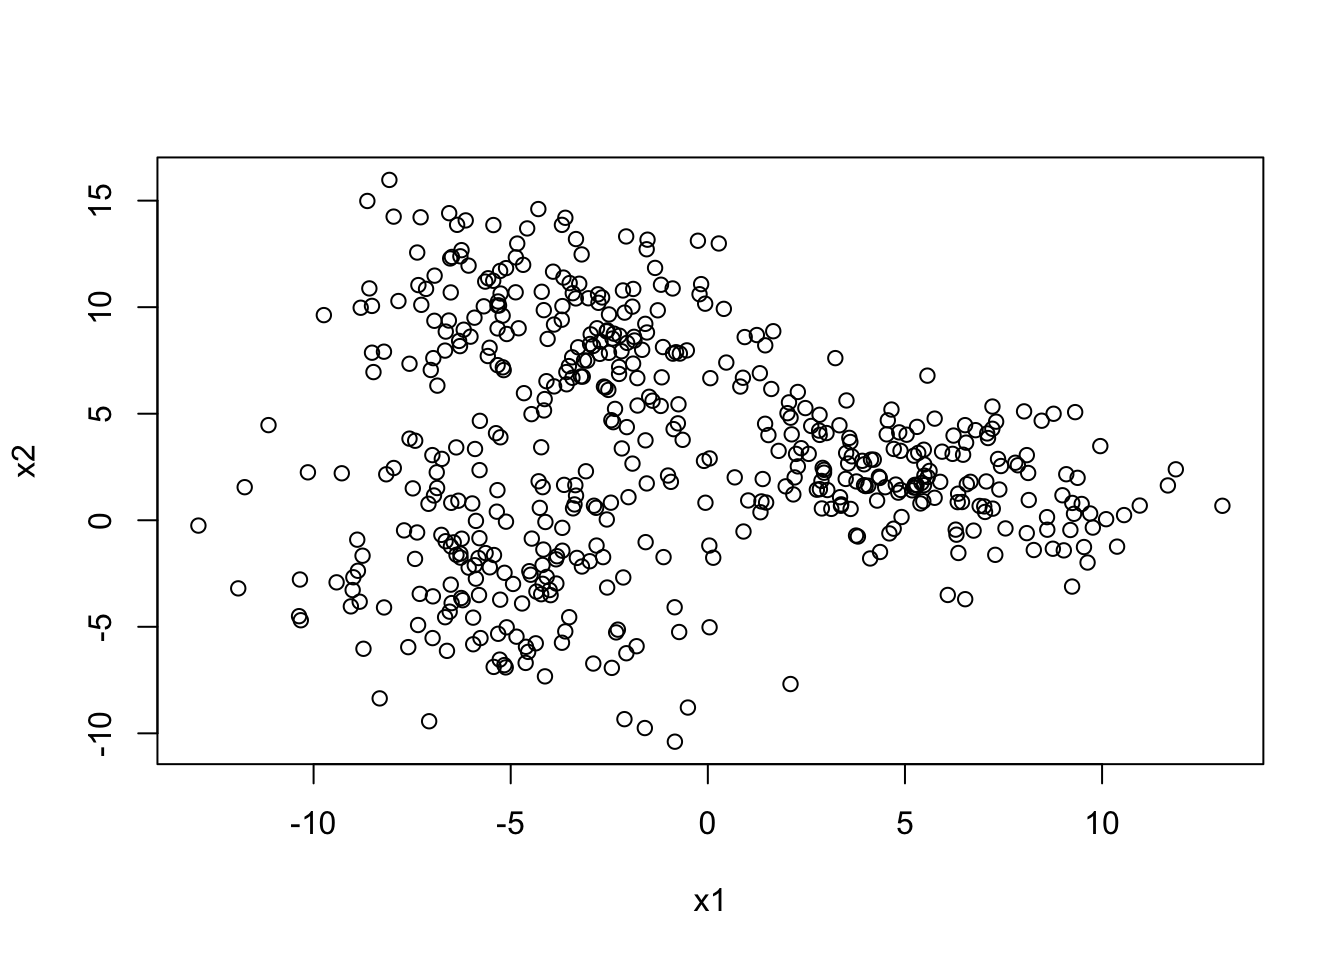
\includegraphics{clusterGen_notes_files/figure-latex/unnamed-chunk-2-1.pdf}

\begin{Shaded}
\begin{Highlighting}[]
\NormalTok{scen1\_1\_plot}
\end{Highlighting}
\end{Shaded}

\begin{verbatim}
## NULL
\end{verbatim}

I am trying to figure out how to assign a color to each cluster for
better visualization, but the problem is that the .mem file has one
fewer row than the .dat file, and I can't figure out how to fix this
without just editing the files on my local machine. So I can't keep
everything on github like I wanted to. I'm still figuring that out, but
in the meantime I used the following code:

\begin{quote}
scen11\_dat \textless-
read.delim(``\url{https://raw.githubusercontent.com/raneyej/clustergen/master/scen1_1.dat}'',
sep = '' ``) scen11\_mem \textless-
read.delim(''\url{https://raw.githubusercontent.com/raneyej/clustergen/master/scen1_1.mem}``,
sep ='' ``) plot\_data \textless- cbind(scen11\_dat, scen11\_mem)
plot(plot\_data\(x1, plot_data\)x2, col = plot\_data\$cluster)
\end{quote}

Hopefully I can figure out a more elegant solution using ggplot in the
future. For now, the plot is on Google Drive.

\textasciitilde\textasciitilde\textasciitilde\textasciitilde\textasciitilde\textasciitilde\textasciitilde\textasciitilde\textasciitilde\textasciitilde\textasciitilde\textasciitilde\textasciitilde\textasciitilde\textasciitilde\textasciitilde\textasciitilde\textasciitilde\textasciitilde\textasciitilde\textasciitilde\textasciitilde\textasciitilde\textasciitilde\textasciitilde\textasciitilde\textasciitilde\textasciitilde\textasciitilde\textasciitilde\textasciitilde\textasciitilde\textasciitilde\textasciitilde\textasciitilde\textasciitilde\textasciitilde\textasciitilde\textasciitilde\textasciitilde\textasciitilde\textasciitilde\textasciitilde\textasciitilde\textasciitilde\textasciitilde\textasciitilde\textasciitilde\textasciitilde\textasciitilde\textasciitilde\textasciitilde\textasciitilde\textasciitilde\textasciitilde\textasciitilde\textasciitilde\textasciitilde\textasciitilde\textasciitilde\textasciitilde\textasciitilde\textasciitilde\textasciitilde\textasciitilde\textasciitilde\textasciitilde\textasciitilde\textasciitilde\textasciitilde\textasciitilde\textasciitilde\textasciitilde\textasciitilde\textasciitilde\textasciitilde\textasciitilde\textasciitilde\textasciitilde\textasciitilde\textasciitilde\textasciitilde\textasciitilde\textasciitilde\textasciitilde\textasciitilde\textasciitilde\textasciitilde\textasciitilde\textasciitilde\textasciitilde\textasciitilde\textasciitilde\textasciitilde\textasciitilde\textasciitilde\textasciitilde\textasciitilde\textasciitilde\textasciitilde\textasciitilde\textasciitilde\textasciitilde{}

Okay now I can't figure out how to `un-name' the column in the .mem
file. I even made a whole new .mem file from scratch to try and fix the
problem and all the sudden R is forcing a name on the column anyway so I
can't rbind. I'm giving up for now. :-(

\end{document}
